\documentclass[../main.tex]{subfiles}
\graphicspath{{../images/}}

\begin{document}

\subsection*{Lecture 1: \hfill  1/16/24}
\hrule \vspace{10px}
\section{Newtons Laws}
\hrule \vspace{10px}

\paragraph{The Four Horsemen of the Apocalypse (In Physics)}
\begin{itemize}
    \item Classical Mechanics
    \item Electromagnetism
    \item Statistical Mechanics
    \item Quantum Mechanics
\end{itemize}

Before 1900, there was no relativity or QM and the world was a simple place \dots

\paragraph{Newton's 1st Law:} The Law of Inertia

And object keeps going unless acted on by a force.

This only applies to and `inertial frame'. 

\paragraph{Newton's 2nd Law:} $\vb{F} = m\vb{a}$

Sum notation: The position vector is
\[
    \vb{r} = (x, y, z) = x(t) \vu{x} + y(t) \vu{y} + z(t) \vu{z}
\] 
in the Cartesian coordinate system. The time derivative gives the velocity
\[
    \vb{v} = \dot{\vb{r}} = \dv{\vb{r}}{t}
\]
and acceleration is the time derivative of velocity
\begin{align*}
    \vb{a} = \dot{\vb{v}} = \ddot{\vb{r}} = \dv[2]{\vb{r}}{t}
\end{align*}
Thus in vector notation, Newton's 2nd law is
\begin{align*}
    m\ddot{\vb{r}} = \vb{F}(\vb{r}, \dot{\vb{r}}, t)
\end{align*}
where $\vb{r}(t)$ is and ordinary differential equation (ODE).

The basic idea of solving mechanics problems is writing down the ODEs and solving them.

\paragraph{What is mass?} $m$ is an `inertial mass'.

In Newton's law of gravity
\begin{align*}
    \vb{F} = -\frac{GMm}{r^2} \vu{r}
\end{align*}
$m$ is the `gravitational mass' and $g \approx \qty{9.8}{\frac{m}{s^2}}$.

A larger mass has a larger inertia or `resistance to being accelerated' (Taylor). Key fact:
When acceleration is zero ($\vb{a} = 0$), the velocity is constant  ($\vb{v} = \text{constant}$).

\paragraph{Momentum:} $\vb{p} = m\vb{v}$

The third law of motion in terms of momentum is
\begin{align*}
    \vb{F} = \dot{\vb{p}} = m\dot{\vb{v}}
\end{align*}

\paragraph{Newton's Third Law:} $\vb{F}_{12} = -\vb{F}_{21}$

In a two body system, the total force of the system is
\begin{align*}
    \vb{F}_t = \vb{F}_{12} + \vb{F}_{21} = 0
\end{align*}
From the second law,
\begin{align*}
    \dot{\vb{p}}_1 = \vb{F}_{21} \qquad \dot{\vb{p}}_2 = \vb{F}_{12}
\end{align*}
adding these two equations gives
\begin{align*}
    \dot{\vb{p}}_1 + \dot{\vb{p}}_2 = 0
\end{align*}
thus the total momentum of the system is conserved.

For a system of $N$ particles, the total momentum is
\begin{align*}
    \dd{t} \sum_i \vb{p}_i = \dv{\vb{p}_{tot}}{t} = \vb{F}_{ext}
\end{align*}
sometimes $\vb{p}_{tot} = \vb{P}$ where the capital $P$ denotes the total momentum of the system.

\newpage
\subsection*{Lecture 2: \hfill  1/18/24}
\hrule \vspace{10px}
\section{A pendulum}
\hrule \vspace{10px}

\paragraph{How to solve a problem:}
\begin{enumerate}
    \item Write down the eq
    \item Solve it
    \item Understand the solution
\end{enumerate}

% figure of pendulum.png
\begin{figure*}[ht]
    \centering
    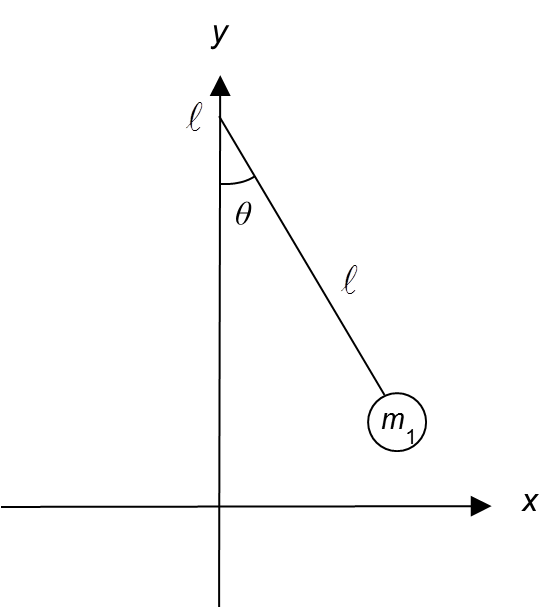
\includegraphics[width=0.4\linewidth]{pendulum.png}
    \caption{A pendulum with mass $m$ and length $l$.}
    \label{fig:2.1}
\end{figure*}    
From Figure \ref{fig:2.1}, we can write down Newton's 2nd law:
\begin{align*}
    \vb{F} &= m\vb{a} = m \ddot{\vb{r}} \\
    F_x &= -mg \sin \theta = m \ddot x \\
    F_y &= -mg \cos \theta + T \cos\theta = m \ddot x
\end{align*}
Using a right triangle we can find the angle using $\tan\theta = x/y$. Furthermore, we can use the
constrain that the length of the pendulum is constant thus $x^2 + y^2 = l^2$. But solving this
system of equations is difficult. Instead we now use a new coordinate system.

\paragraph{Quick Hack} Using the arc length $l = L\theta$ and choosing a coordinate in the direction
of the pendulums path, we can write the force equation as
\begin{align*}
    F_l = -mg \sin\theta = m \ddot l = m L \ddot \theta
\end{align*}
Thus the equation of motion is
\begin{align*}
    \ddot \theta = -\frac{g}{L} \sin\theta
\end{align*}
which is a second order ODE. This can only be solved with two conditions. We can use the initial
conditions (at $t = 0$) of the position $\theta(t = 0) = \theta_0$ and velocity $\dot\theta(0) = 0$.

\paragraph{Polar Coordinates} From Taylor:

\begin{align*}
    x &= r \cos\phi \\
    y &= r \sin\phi
\end{align*}
For an arbitrary vector $\vb{v}$ it has the Cartesian vector components
\begin{align*}
    \vb{v} = v_x \vu{x} + v_y \vu{y}
\end{align*}
Where the magnitude of the unit vectors are equivalent:
\begin{align*}
    \abs{\vu{x}} = \abs{\vu{y}} = 1
\end{align*}
and the magnitude of the vector is
\begin{align*}
    \abs{\vb{v}} &= \sqrt{\vb{v} \cdot \vb{v}} \\
    &= \sqrt{v_x^2 \vu{x} \cdot \vu{x} + 2 v_x v_y \vu{x} \cdot \vu{y} v_y^2 \vu{y} \cdot \vu{y}}\\
    &= \sqrt{v_x^2 + v_y^2}
\end{align*}
The vector $\vb{v}$ can be written in polar coordinates as
\begin{align*}
    \vb{v} = v_r \vu{r} + v_\phi \vu{\phi}
\end{align*}
where radial vector is
\begin{align*}
    \vb{r} = r \vu{r}, \qquad \vu{r} = x \vu{x} + y \vu{y}
\end{align*}
taking the time derivative of $\vb{r}$ gives the velocity
\begin{align*}
    \dot{\vb{r}} = \dot{r} \vu{r} + r \dot{\vu{r}} 
\end{align*}
but how do we find $\dot{\vu{r}}$? We can look at the change in the direction of the radial unit
vector for a small change in time $\Delta t$. Thus,
\begin{align*}
    \Delta \vu{r} \approx r \Delta\phi \vu*{\phi}
\end{align*}
dividing both sides by $\Delta t$ gives
\begin{align*}
    \frac{\Delta \vu{r}}{\Delta t} \approx r \frac{\Delta \phi}{\Delta t} \vu*{\phi}
    = r \dot\phi \vu*{\phi}
\end{align*}
Therefore, the vector in polar coordinates is
\begin{align*}
    \dot{\vb{r}} = \dot{r} \vu{r} + r \dot\phi \vu*{\phi} = v_r \vu{r} + v_\phi \vu*{\phi}
\end{align*}
where the polar components $v_r$ and $v_\phi$ are related to the radial and angular velocity
respectively. Taking the time derivative of $\dot{\vb{r}}$ gives the acceleration
\begin{align*}
    \ddot{\vb{r}} &= \ddot r \vu{r} + \dot r \dot{\vu{r}} + \dot r \dot\phi \vu{\phi} + 
    r \ddot\phi \vu{\phi} + r \dot\phi \dot{\vu\phi} \\
    &= \dot{v}_r \vu{r} + v_r \dot{\vu{r}} + \dot{v}_\phi \vu*{\phi} + v_\phi \dot{\vu*{\phi}}
\end{align*}

\newpage
\subsection*{Lecture 3: \hfill  1/22/24}
\hrule \vspace{10px}
\section{Polar Coordinates}
\hrule \vspace{10px}

using the geometric relation $\dot{\vu*{\phi}} = -\dot\phi \vu{r}$, we can write the acceleration as
\begin{align*}
    \ddot{\vb{r}} &= (\ddot r - r \dot\phi^2) \vu{r} + (r \ddot\phi + 2r \ddot\phi) \vu*{\phi} \\
    &= a_r \vu{r} + a_\phi \vu*{\phi}
\end{align*}
where $r\dot\phi^2 = r\omega^2$ is the centripetal acceleration and $r\ddot\phi = r \dot \omega$ is
the tangential acceleration.

From the Pendulum problem we know that the string is taut $r = L$ thus the radial velocity is zero
$\dot r = 0$. Thus the force equation in the $\vu*{\phi}$ direction is
\begin{align*}
    F_\phi &= m L \ddot\phi = -mg \sin\theta \\
    \ddot\phi &= -\frac{g}{L} \sin\theta
\end{align*}
which is the same equation of motion. 

\paragraph{Projectile in 2D} The initial conditions of a general projectile is usually
\begin{align*}
    F_x &= 0 = m\ddot x \\
    F_y &= -mg = m\ddot y
\end{align*}
thus the equations of motion are
\begin{align*}
    \ddot x &= 0 \\
    \ddot y &= -g
\end{align*}
And solving these equations gives the position of the projectile
\begin{align*}
    x(t) &= v_{ox} t \\
    y(t) &= y_o v_{oy} t - \frac{1}{2} g t^2
\end{align*}

This can be expanded on with the addition of air resistance $\vb{f}$. This drag force is
proportional to the velocity:
\begin{align*}
    \vb{f} \propto -\vu{v}
\end{align*}
and there are two types of air resistance: linear
\begin{align*}
    \vb{f}_l = -bv \vu{v} = -b \vb{v}
\end{align*}
and quadratic
\begin{align*}
    \vb{f}_q = -cv^2 \vu{v}
\end{align*}
where we compare the terms with
\begin{align*}
    \frac{f_l}{f_q} = \frac{cv}{b}
\end{align*}

\paragraph{Linear} $\vb{f}_l = -b \vb{v}$

From Newton's 2nd law
\begin{align*}
    F_x &= -bv_x = m\ddot x = m \dot v_x \\
    F_y &= -mg - bv_y = m\ddot y = m \dot v_y
\end{align*}
For the case of uncoupled differential equations (such as pure horizontal motion), we can solve the
horizontal equation
\begin{align*}
    \dot v_x = -\frac{b}{m} v_x 
\end{align*}
which has a general solution
\begin{align*}
    v_x = A e^{-kt}
\end{align*}
where
\begin{align*}
    k = \frac{b}{m}, \quad A = v_{ox}
\end{align*}
to find the position we have to integrate $\dot x = v_x$:
\begin{align*}
    x &= x_o + \int_0^t v_x(t') \dd{t'} \\
    &= x_o + \qt[-\frac{v_{xo}}{k} e^{-kt}]\eval_0^t
\end{align*}
where we have a limit of $t \rightarrow \infty$

For pure vertical motion, we solve the equation
\begin{align}
    \dot v_y = -g - \frac{b}{m} v_y
\end{align}
and with the initial condition $\dot v_y = 0$ we can solve for the velocity
\begin{align*}
    v_y = -\frac{mg}{b} = v_{ter}
\end{align*}
where $v_{ter}$ is the terminal velocity. To get position, we use a trick by rewriting the equation
as
\begin{align*}
    m\dot v_y = -mg - bv_y = -mg - b(v_y - v_{ter})
\end{align*}
and we can solve similar to the horizontal case using the general solution
\begin{align*}
    v_y - v_{ter} = A e^{-kt} = (v_{oy} - v_{ter}) e^{-kt}bye 
\end{align*}

\newpage
\subsection*{Lecture 4: \hfill  1/24/24}
\hrule \vspace{10px}
\section{Air Resistance}
\hrule \vspace{10px}

\paragraph{Last time:}
\begin{align*}
    \vb{f}_l &= -b \vb{v} \quad \dot{\vb{r}} = \vb{v} \\
    \vb{f}_q &= -cv^2 \vu{v}
\end{align*}
In the case of linear, $x$ motino has a range, $y$ velocity has a terminal velocity $v_t$.

\paragraph{Horizontal Quadratic Drag}
\begin{align*}
    F_y &= -mg - c\abs{v_y} v_y \\
    m\ddot y &= F_y \\
    m\dot v_y &= -mg - c\abs{v_y} v_y
\end{align*}
when $v_y = 0$ we have the terminal velocity
\begin{align*}
    v_{ter} = \sqrt{\frac{mg}{c}} \qor c = \frac{mg}{v_{ter}^2}
\end{align*}
thus the equation of motion is
\begin{align*}
    \dot v_y = -g - \frac{c}{m} v_y^2 = -g(1 - \frac{v_y^2}{v_{ter}^2}) = \dv{v_y}{t}
\end{align*}
using separation of variables
\begin{align*}
    \frac{1}{1 - \frac{v_y^2}{v_t^2}} \dd{v_y} = -g \dd{t}
\end{align*}
integrating both sides
\begin{align*}
    \int_{v_{oy}}^{v_y} \frac{1}{1 - \frac{v_y^2}{v_t^2}} \dd{v_y} = -g \int_0^t \dd{t}
\end{align*}
where we get the integral using the hyperbolic tangent
\begin{align*}
    v_t \arctanh{\frac{v_y}{v_t}} &= -gt \\
    v_y &= -v_t \tanh(gt)
\end{align*}

\paragraph{2D Motion} For Quadratic
\begin{align*}
    F_x &= -c v v_x = -c \sqrt{v_x^2 + v_y^2} v_x  = m\dot v_x \\
    F_y &= -mg - c v v_y = -mg - c \sqrt{v_x^2 + v_y^2} v_y = m \dot v_y
\end{align*}
where $v = \sqrt{v_x^2 + v_y^2}$. For linear, it is simply
\begin{align*}
    F_x &= -bv_x = m\dot v_x \\
    F_y &= -mg - bv_y = m\dot v_y
\end{align*}

% lecture 1/26/24
\pagebreak
\subsection*{Lecture 5: \hfill  1/26/24}
\hrule \vspace{10px}
\section{Center of Mass}
\hrule \vspace{10px}

For $N$ particles, the center of mass is
\begin{align*}
    \vb{R} = \frac{1}{M} \sum_i m_i \vb{r}_i
\end{align*}
where $M = \sum_i m_i$ is the total mass of the system. This is similar to the `weighted' average!
Taking the time derivative of $\vb{R}$ gives the total momentum
\begin{align*}
    \dot{\vb{R}} = \frac{1}{M} \sum_i m_i \dot{\vb{r}}_i = \frac{1}{M} \sum_i \vb{p}_i = \vb{P}
\end{align*}
From Newton's 3rd Law
\begin{align*}
    \sum \dot{\vb{p}}_i = \vb{F}_{ext}
\end{align*}
and from the second Law
\begin{align*}
    M \ddot{\vb{R}} = \vb{F}_{ext}
\end{align*}
in integral form 
\begin{align*}
    \vb{R} = \frac{1}{M} \int \vb{r} \dd{m}
\end{align*}
and using the mass density $\dd{m} = \rho \dd{V}$ we can write
\begin{align*}
    \vb{R} = \frac{1}{M} \int \vb{r} \rho \dd{V} = \frac{1}{M} \int \vb{r} \rho \dd{x} \dd{y} \dd{z}
\end{align*}
For a uniform solid semisphere lying on the $xy$ plane with radius $R=1$ and mass $M = 2\pi/3$, the
CM is 
\begin{align*}
    z &= \frac{1}{M} \int \rho z \dd{m} \\
    &= \frac{1}{M} \int z\pi r^2 \dd{z} \\
    &= \frac{1}{M} \int_0^1 \pi z (1 - z^2) \dd{z} \\
    &= \frac{\pi}{M} \qt[\frac{1}{2} - \frac{1}{4}] = \frac{3}{8}
\end{align*}
\subsubsection*{Angular Momentum}
For the singular particle, the angular momentum is
\begin{align*}
    \vb{l} = \vb{r} \cross \vb{p}
\end{align*}
and the total angular momentum of an multi particle system is
\begin{align*}
    \vb{L} = \sum_i \vb*{\ell}_i = \sum_i \vb{r}_i \cross \vb{p}_i
\end{align*}
and the time derivative of $\vb{L}$ is
\begin{align*}
    \dot{\vb{L}} = \sum_i \dot{\vb{r}}_i \cross \vb{p}_i + \vb{r}_i \cross \dot{\vb{p}}_i
    = \sum_i \vb{r}_i \cross \dot{\vb{p}}_i = \sum_i \vb{r}_i \cross \vb{F}_i = \sum_i \vb{\Gamma}_i
\end{align*}
where $\dot{\vb{r}}_i \cross \vb{p}_i = 0$ since $\dot{\vb{r}}_i$ is parallel to $\vb{p}_i$. Since
$\vb{F}_i$ is the force on the $i$th particle,
\begin{align*}
    \vb{F}_i = \sum_{j\neq i} \vb{F}_{ij} + \vb{F}_i^{ext}
\end{align*}
Plugging into the time derivative of angular momentum
\begin{align*}
    \dot{\vb L} = \sum_i \sum_{j\neq i} \vb{r}_i \cross \vb{F}_{ij} + \sum_i \vb{F}_i^{ext}
\end{align*}
In terms of a matrix, the double sum skips the diagonal elements and thus we can pair the indices
that are reflected on the diagonal
\begin{align*}
    \sum_i \sum_{j > i} (\vb r_i \cross \vb F_{ij} + \vb r_j \cross \vb F_{ji}) = \sum_i \sum_{j > i}
    (\vb r_i - \vb r_j) \cross \vb F_{ij}
\end{align*}
where we use the associativity of the cross product and N3L $\vb{F}_{ij} = -\vb{F}_{ji}$. In
addition the force must be central along the line connecting the two particles. Thus we get
\begin{align*}
    \dot{\vb L} = \sum_i \Gamma_i^{ext}
\end{align*}
The direction of the angular momentum is along the axis of rotation. 

\paragraph{A car} To move a car forward, you exert a torque clockwise on the wheels, and from the 
conservation of angular momentum the car will typically want to rotate counter clockwise which feels
like the weight is being pushed back. The torque on the car will increase the friction on the rear
wheel (increasing traction) and thus RWD are better at high accelerations.

% lecture 1/29/24
\pagebreak
\subsection*{Lecture 6: \hfill  1/29/24}
\hrule \vspace{10px}
\section{Energy}
\hrule \vspace{10px}

Review: There are two requirements for conservation of angular momentum
\begin{enumerate}
    \item Force is central
    \item External torque is zero
\end{enumerate}

\paragraph{Kinetici Energy:} $T = \frac{1}{2} m v^2 = \frac{1}{2} \vb{v} \cdot \vb{v}$. Taking the
time derivative
\begin{align*}
    \dot T &= \frac{1}{2} (\dot{\vb{v}} \cdot \vb{v} + \vb{v} \cdot \dot{\vb{v}}) \\
    &= m \dot{\vb{v}} \cdot \vb{v} = \vb{F} \cdot \vb{v}
\end{align*}
and integrating over time $t_1$ to $t_2$
\begin{align*}
    \int_{t_1}^{t_2} \dot T \dd{t} = \Delta T = \int_{t_1}^{t_2} \vb{F} \cdot \vb{v} \dd{t}
    = \int_{t_1}^{t_2} \vb{F} \cdot \dd{\vb{r}} = W(1 \to 2)
\end{align*}
since $\vb{v} \cdot \dd{t} = \dd{\vb{r}}$ and $\vb{F} \cdot \dd{\vb{r}}$ hints that this is a line
integral.

\paragraph{Example:}
\begin{align*}
    \vb{F}(x,y) &= \vb{r} = x \vu{x} + y \vu{y} \\
    \dd{vb{r}} &= \dd{x} \vu{x} + \dd{y} \vu{y}
\end{align*}
(a) $y = x$ from $a = (0,0)$ to $b = (1,1)$
\begin{align*}
    \int_a^b \vb{F} \cdot \dd{\vb{r}} &= \int_0^1 (x \dd{x} + y \dd{y}) \\
    &= \int_0^1 x \dd{x} + \int_0^1 x \dd{x} = 1
\end{align*}
(b) $y = x^2$ and $\dd{y} = 2x \dd{x}$
\begin{align*}
    \int_a^b \vb{F} \cdot \dd{\vb{r}} &= \int_0^1 (x \dd{x} + x^2 \dd{y}) \\
    &= \int_0^1 x \dd{x} + \int_0^1 2x^2 \dd{x} = 1
\end{align*}
thus the line integral is independent of the path.
\subsubsection*{Conservative force}
\begin{enumerate}
    \item Given $\vb{F}(\vb{r})$, there is no dependence on $\vb{v}$, $t$.
    \item $\int \vb{F} \cdot \dd{\vb{r}}$ is independent of the path.
\end{enumerate}
\begin{align*}
    U(\vb{r}) = -W (\vb{r}_0 \to \vb{r}) = -\int_{\vb{r}_0}^{\vb{r}} \vb{F} \cdot \dd{\vb{r}}'
\end{align*}
For gravity
\begin{align*}
    U_g (\vb{r}) = - \int_a^b \vb{F}_g \cdot \dd{\vb{r}} = - \int_a^b -mg \dd{y}' = mg(y_a - y_b)
\end{align*}
\paragraph{Work-Kinetic Energy Theorem:}
\begin{align*}
    W(1 \to 2) = W(1 \to \mathcal{O}) + W(\mathcal{O} \to 2) = U(1) - U(2) = \Delta T
\end{align*}
From this we have
\begin{align*}
    \Delta T = T_2 - T_1 = U_1 - U_2
\end{align*}
rearranging terms give the mechanical energy
\begin{align*}
    T_2 + U_2 = T_1 + U_1 = E
\end{align*}
and for $N$ conservative forces in a system
\begin{align*}
    E = T + U_1 + U_2 + \dots + U_N
\end{align*}

\pagebreak
\subsection*{Lecture 7: \hfill  1/31/24}
\hrule \vspace{10px}
\section*{Energy Part 2}
\hrule \vspace{10px}

\paragraph{Conservative Force: Potential Energy} The mechanical energy
\begin{align*}
    E = T + U
\end{align*}
is made up of the sum of the kinetic and potential energy. This is useful for
\begin{itemize}
    \item obtaining equations of motion (EOM)
\end{itemize}
e.g. finding the EOM for a simple pendulum of mass $m$, length $L$ and initial angle $\theta$. The
kinetic energy is
\begin{align*}
    T = \frac{1}{2} m L^2 \dot{\theta}^2
\end{align*}
where the magnitude of velocity is the tangential component $v = L \omega = L \dot \theta$. The 
potential energy is
\begin{align*}
    U = -mgy = -mg L \cos\theta
\end{align*}
and the conservation of energy tells us that the mechanical energy is constant
\begin{align*}
    T + U = \textrm{constant} &= E \\
    \frac{1}{2} m L^2 \dot{\theta}^2 - mg L \cos\theta &= E
\end{align*}
and in the intial condition we know that the velocity is zero $\dot{\theta} = 0$ and thus 
\begin{align*}
    -mg L \cos\theta_{max} &= E
\end{align*}
taking the time derivative of the energy equation gives
\begin{align*}
    m L^2 \dot{\theta} \ddot{\theta} + mg L \sin\theta \dot{\theta} &= 0 \\
    \ddot{\theta} + \frac{g}{L} \sin\theta &= 0 \\
    \ddot \theta &= -\frac{g}{L} \sin\theta
\end{align*}
taking the time derivative of the energy is a useful trick for finding the EOM when we are trying to
solve for $\dot{v}^2$.

\paragraph{Last time} we found the potential energy for a position $\vb{r}$ in a conservative force
field $\vb{F}(\vb{r})$ is
\begin{align*}
    U(\vb{r}) = -W(\vb{r}_0 \to \vb{r}) = -\int_{\vb{r}_0}^{\vb{r}} \vb{F} \cdot \dd{\vb{r}}'
\end{align*}
from the fundamental theorem of calculus (derivatives and intergrals are inverses) we want to find
a function where the derivative equals the conservative force: First we take an infinitesimal change
in the position $\vb{r} \to \vb{r} + \dd{\vb{r}}$ and the change in potential energy is
\begin{align*}
    U(\vb{r} + \dd{\vb{r}}) &= - \int_{\vb{r}_0}^{\vb{r} + \dd{\vb{r}}} \vb{F} \cdot \dd{\vb{r}}' \\
    &= - \int_{\vb{r}_0}^{\vb{r}} \vb{F} \cdot \dd{\vb{r}}' - \int_{\vb{r}}^{\vb{r} + \dd{\vb{r}}}
    \vb{F} \cdot \dd{\vb{r}}' \\
    &= U(\vb r) - F(\vb r) \cdot \dd{\vb{r}}
\end{align*}
where is know that the force is constant over a small distance. Moving the terms gives
\begin{align*}
    U(\vb{r} + \dd{\vb{r}}) - U(\vb{r}) &= - \vb{F} \cdot \dd{\vb{r}} \\
    &= - (F_x \dd{x} + F_y \dd{y} + F_z \dd{z})
\end{align*}
where we use Cartesian Coordinates, and we know that the gradient of potential is
\begin{align*}
    \grad U &= \vu{x} \pdv{U}{x} + \vu{y} \pdv{U}{y} + \vu{z} \pdv{U}{z} \\
    &= - (F_x \vu{x} + F_y \vu{y} + F_z \vu{z}) = - \vb{F}
\end{align*}

\paragraph{Example 3: 1D motion} If we know what $U$ is as a function of $x$, we can find the force!
At points where $E = U$ we call these classical turning points. At a region of a relative minimum, 
a particle below the threshold of the turning point will oscillate between the two turning points.
And at $E>U_max$ the particle is unbound and will escape the forces that attracted it.

\paragraph{Example 4:}
\begin{align*}
    E &= T + U(x) \textrm{ is constant} \\
    T &= \frac{1}{2} m \dot{x}^2  = E - U(x) \\
    \dot {x}^2 &= \frac{2}{m} (E - U(x)) \\
    \dot{x} &= \pm \sqrt{\frac{2}{m} (E - U(x))}
\end{align*} 
using seperation of variables
\begin{align*}
    \dv{x}{t} &= \sqrt{\frac{2}{m} (E - U(x))} \\
    \sqrt{\frac{m}{2}} \dd{t} &= \frac{\dd{x}}{\sqrt{E - U(x)}} \\
    \int_{t_1}^{t_2} \sqrt{\frac{m}{2}} \dd{t} &= \int_{x_1}^{x_2} \frac{\dd{x}}{\sqrt{E - U(x)}} \\
    (t_2 - t_1) &= \sqrt{\frac{2}{m}} \int_{x_1}^{x_2} \frac{\dd{x}}{\sqrt{E - U(x)}}
\end{align*}
where the sign of the velocity is positive within the oscillating bounds of the turning points and
changes sign as the particle moves past the turning point. 

\pagebreak
\subsection*{Lecture 8: \hfill  2/2/24}
\hrule \vspace{10px}
\section*{Energy cont'd}

\paragraph{Last time:} Conservative force as a negative gradient of potential:
\[
    \vb{F} = -\grad U
\]
with classical turning points at $E = U$.

\paragraph{Conditions of a conservative force}
\begin{itemize}
    \item Only depends on position $\vb{r}$ (or just constant)
    \item Work done is path independent (this is sometimes hard to check) $\Leftrightarrow
    \curl{\vb F} = 0$
\end{itemize}

\paragraph{What is curl?} In 3D Cartesian coordinates
\begin{align*}
    \curl{\vb F} &= \mqty| \vu{x} & \vu{y} & \vu z \\
                        \pdv{x} & \pdv{y} & \pdv{z} \\
                        F_x & F_y & F_z | \\
    &= \qt(\pdv{F_z}{y} - \pdv{F_y}{z}\vu{x} + \pdv{F_x}{z} - \pdv{F_z}{x}\vu{y} +
    \pdv{F_y}{x} - \pdv{F_x}{y}\vu{z}\qt)
\end{align*}
Mathematically we know that if the force vector is a gradient of a scalar potential
\begin{align*}
    \vb{F} = \grad{\phi} = - \grad{U} \quad \Leftrightarrow \quad \curl{\vb{F}} = 0
\end{align*}
The curl of a gradient is always zero! Short `proof':
\begin{align*}
    F_x = -\pdv{U}{x} \quad F_y = -\pdv{U}{y} \quad F_z = -\pdv{U}{z}
\end{align*}
and the curl
\begin{align*}
    \mqty| \vu{x} & \vu{y} & \vu z \\
    \pdv{x} & \pdv{y} & \pdv{z} \\
    -\pdv{U}{x} & -\pdv{U}{y} & -\pdv{U}{z} | = 0
\end{align*}
Proving that the line integral is path independent is a little difficult, but in general we know
that the two different paths $a$ and $b$ from points $1$ to $2$ we can write the work as
\begin{align*}
    \int_1^2 \vb{F} \cdot \dd{\vb{r}_2} - \int_1^2 \vb{F} \cdot \dd{\vb{r}_1} 
    = \oint_{a-b} \vb{F} \cdot \dd{\vb{r}} = \int_A (\curl \vb{F}) \cdot \dd{\vb{A}} = 0
\end{align*}
where we invoke Stokes' Theorem to find the integral of the curl over the surface $A$ is zero.

\paragraph{Conservative Force:} \( \vb{F} = x \vu{x} + y \vu{y} \) is conservative, but is
\begin{align*}
    \vb{F}(\vb{r}) = F(\vb{r}) \vu{r} 
\end{align*} 
a central force always conservative? We will need to check the curl of the force to find out. But
first we define spherical coordinates $(r, \theta, \phi)$
\begin{align*}
    x &= r \sin\theta \cos\phi \\
    y &= r \sin\theta \sin\phi \\
    z &= r \cos\theta
\end{align*}
and the central force in spherical coordinates is
\begin{align*}
    \vb{F} = F(\vb{r}) \vu{r} + 0 \vu{\theta} + 0 \vu{\phi}
\end{align*}
the curl in spherical coordinates is
\begin{align*}
    \curl \vb{F} &= \frac{1}{r^2 \sin\theta} \qt[\pdv{\theta} (F_\phi \sin\theta) - \pdv{F_\theta}{\phi}] \vu{r}\\
    &+ \frac{1}{r} \qt[\frac{1}{\sin\theta} \pdv{F_r}{\phi} - \pdv{r} (r F_\phi)] \vu{\theta} \\
    &+ \frac{1}{r} \qt[\pdv{r} (r F_\theta) - \pdv{F_r}{\theta}] \vu{\phi}
\end{align*}
And since
\begin{align*}
    \pdv{F}{\theta} = \pdv{F}{\phi} = 0
\end{align*}
the curl is zero $\curl \vb{F} = 0$ and thus $\vb{F}$ is a conservative central force.

\paragraph{Gravity Conservative?} The force due to gravity
\begin{align*}
    \vb{F}_g = -\frac{G M m}{r^2} \vu{r} = -\frac{G M m}{r^3} \vb{r}
\end{align*}
is a central force as it only depends on $\vb{r}$. e.g. for a a two mass system:
\begin{align*}
    \vb{F}_{12} = - \frac{G m_1 m_2}{\abs{\vb{r}_1 - \vb{r}_2}^3} (\vb{r}_1 - \vb{r}_2)
\end{align*}
Using Translational Invariance, we can shift the origin to the center of $m_2$
\begin{align*}
    \vb{r}_2 &= 0 \quad \vb{F}_{12} = - \frac{G m_1 m_2}{\vb{r}_1^3} \vb{r}_1
\end{align*}
or
\begin{align*}
    F_{12} = - \grad_1 U = - (\pdv{U}{x_1}, \pdv{U}{y_1}, \pdv{U}{z_1})
\end{align*}
where the potential energy due to the interaction between 1 and 2 is
\begin{align*}
    U_{12} = - \frac{G m_1 m_2}{\abs{\vb{r}_1 - \vb{r}_2}}
\end{align*}
from newtons 3rd law, the force on 2 due to 1 is
\begin{align*}
    \vb{F}_{12} = - \vb{F}_{21}
\end{align*}
so
\begin{align*}
    -\grad_1 U_{12} &\to \vb{F}_{21} = \grad_1 U_{12} \\
    \grad_1 U_{12} (\vb{r}_1 0 \vb{r}_2) &= - \grad_2 U_{12} (\vb{r}_2 0 \vb{r}_1) \\
    u_{12}(\vb{x}) &\quad \vb{x} = \vb{r}_1 - \vb{r}_2 \\
    \grad_1 U_{12}(\vb{x}) &= \grad_x U_{12}(\vb{x}) = - \grad_2 U_{12}(\vb{x})
\end{align*}
so
\begin{align*}
    \vb{F}_{12} = - \grad_1 U_{12} \qquad \vb{F}_{21} = - \grad_2 U_{12}
\end{align*}
and for $N$ particles
\begin{align*}
    \vb{F}_i = - \grad_i U \qquad U = \sum_{i,j} U_{ij} + \sum_i U_i^{\text{ext}}
\end{align*}

\newpage
\subsection*{Lecture 9: \hfill  2/5/24}
\hrule \vspace{10px}
\section{Oscillations}

\& Simple Harmonic Oscillators For the simple case of a mas on a spring, the spring force is
$F_{s} = -k(x - x_o)$
where the force is conservative and the (elastic) potential energy is
$U_s = \frac{1}{2} k (x - x_o)^2$.

\paragraph*{Aribtrary Potential energy} 
% insert fig
\begin{figure}[ht]
    \centering
    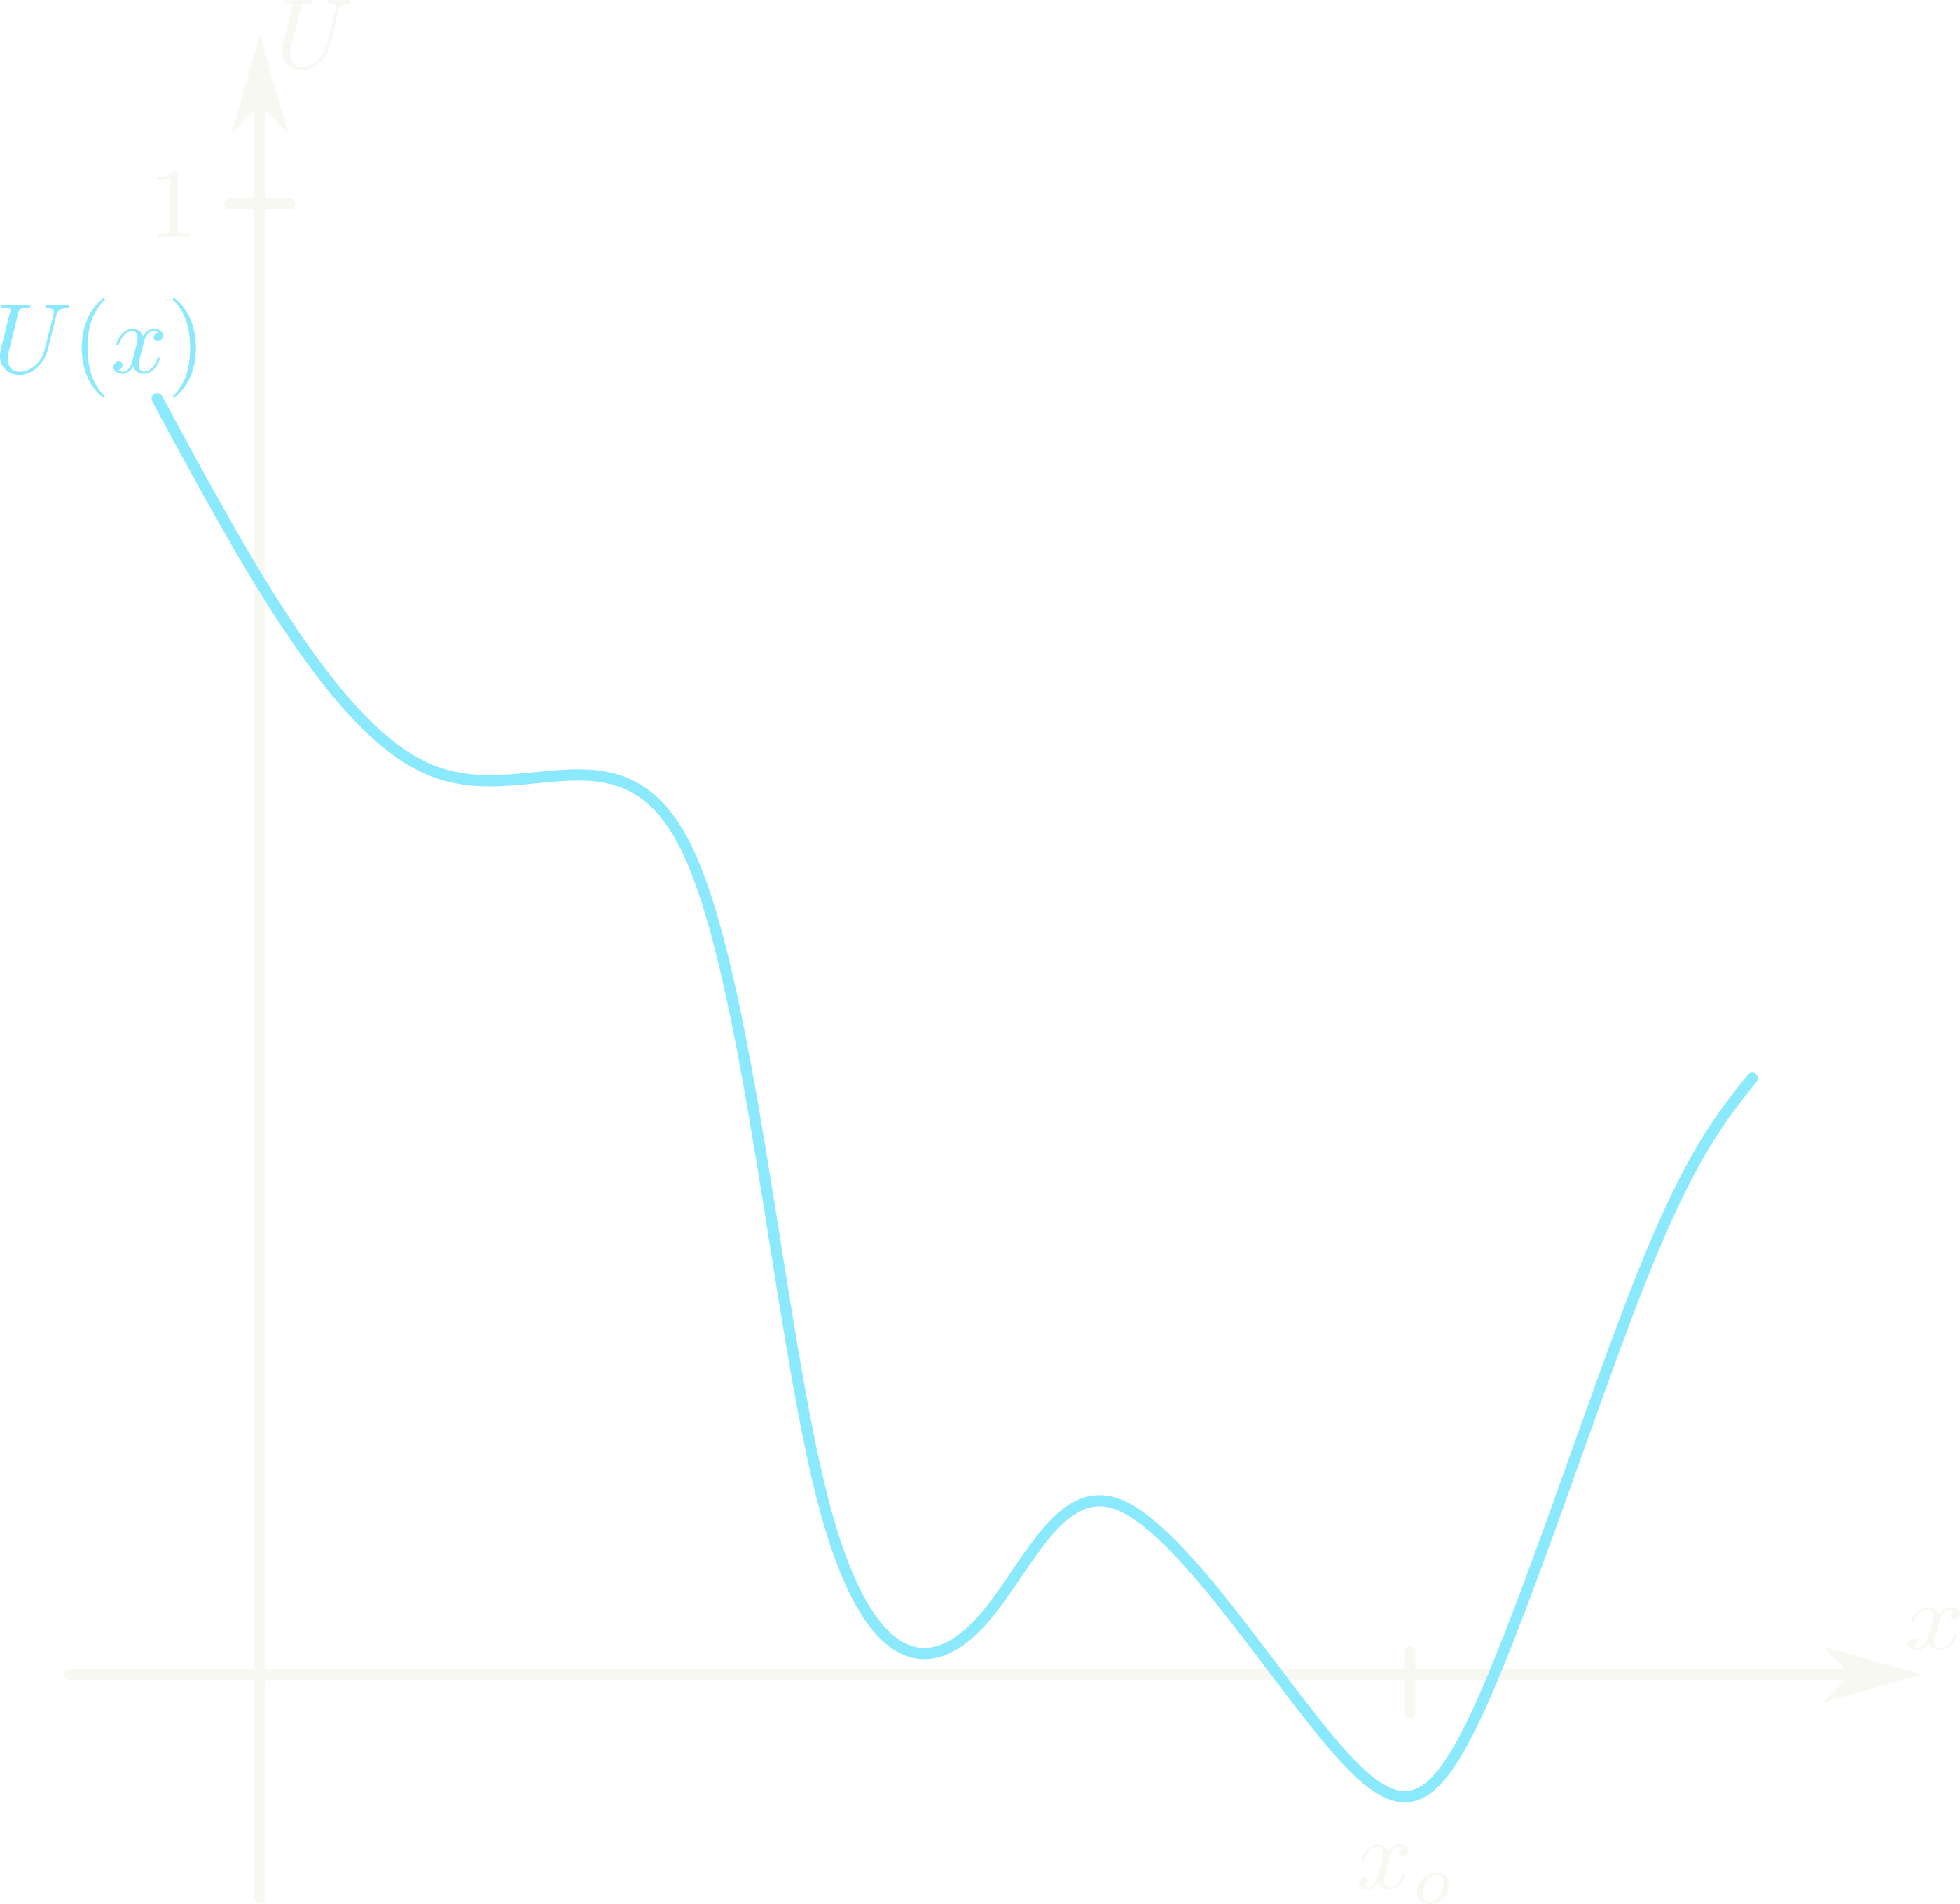
\includegraphics[width=0.5\textwidth]{5_1.png}
    \caption{Arbitrary Potential Energy: $\vb{F} = - \grad U$}
    \label{fig:fig1}
\end{figure}

FOr a equilibrium positon $x_o$ we can take the taylor expansion of the potential energy
\begin{align*}
    U(x) = U(x_o) + U' (x_o) \Delta x + \frac{1}{2} U''(x_o) \Delta x^2 + \dots
\end{align*}
where $\Delta x = x - x_o$. Setting $x_o$ to the reference point of $U$ cancels the first term and
the conservative nature tells us that the second term is also zero thus we are left with the third
term where the spring constant is
\begin{align*}
    k = U'' (x_o)
\end{align*}
To find the equations of motion, using N2L
\begin{align*}
    m\ddot x &= F = - k (x - x_o) \\
    \ddot x &= - \frac{k}{m} (x - x_o)
\end{align*}
where we have a constant of angular frequency
\begin{align*}
    \omega_o = \sqrt{\frac{k}{m}}
\end{align*}
the solution could be a sinusoidal function
\begin{align*}
    x(t) \approx \sin \omega_o t 
\end{align*}
but we are missing the initial value, so
\begin{align*}
    x(t) \approx \sin \omega_o t + x_o
\end{align*}
the general solution is linear combinations of the sine and cosine functions
\begin{align*}
    x(t) &= A \sin \omega_o t + B \cos \omega_o t + x_o \\
    \dot x(t) &= \omega_o A \cos \omega_o t - \omega_o B \sin \omega_o t
\end{align*}
where we need 2 initial conditions to solve for $A$ and $B$. e.g. $x(0)$ and $\dot x(0)$.
\begin{align*}
    B &= x(0) - x_o = \Delta x(0), \qquad A = \frac{\dot x(0)}{\omega_o}
\end{align*}

\paragraph*{Euler's Solution} We can also use a general solution of the form
\begin{align*}
    e^{i \theta} = \cos \theta + i \sin \theta
\end{align*}
where
\begin{align*}
    \abs {e^{i \theta}} = \cos^2 \theta + \sin^2 \theta = 1
\end{align*}
taking the derivatives
\begin{align*}
    \dv{t} e^{i \omega_o t} &= i \omega_o e^{i \omega_o t} \\
    \dv[2]{t} e^{i \omega_o t} &= - \omega_o^2 e^{i \omega_o t}
\end{align*}
and the general solution is
\begin{align*}
    x(t) &= A e^{i \omega_o t} + B e^{-i \omega_o t} + x_o
\end{align*}
this does not mean that we have an imaginary solution, but rather we are using the geomtric 
nature of the solution. 

\paragraph*{Third Way} We can also use a method where we introduce the phase
\begin{align*}
    x(t) &= A \cos(\omega_o t - \delta) + x_o \\
    \dot x(t) &= -A \omega_o \sin(\omega_o t - \delta)
\end{align*}
for $t = 0$ we have
\begin{align*}
    x(0) &= A \cos(-\delta) + x_o = A \cos \delta + x_o \\
    \dot x(0) &= -A \omega_o \sin(-\delta) = A \omega_o \sin \delta
\end{align*}
and the constants are found by squaring and adding the two equations
\begin{align*}
    A^2 &= (x(0) - x_o)^2 + \frac{\dot x(0)^2}{\omega_o^2}
        = \Delta x(0)^2 + \frac{\dot x(0)^2}{\omega_o^2}\\
    \delta &= \arctan \frac{\dot x(0)}{\omega_o (x(0) - x_o)}
        = \arctan \frac{\dot x(0)}{\omega_o \Delta x(0)}
\end{align*}

\paragraph*{Energy of the Oscillator} The mechanical energy is $E = T + U$
\begin{align*}
    T &= \frac{1}{2} m \dot x^2 = \frac{1}{2} m \omega_o^2 A^2 \sin^2(\omega_o t - \delta) \\
    U &= \frac{1}{2} k (x - x_o)^2 = \frac{1}{2} k A^2 \cos^2(\omega_o t - \delta)
\end{align*}
setting $x_o = 0$ we can work with a much simple case
\begin{align*}
    U &= \frac{1}{2} k x^2 \\  
    T &= \frac{1}{2} k x^2
\end{align*}
using the third way where
\begin{align*}
    x(t) &= A \cos(\omega_o t - \delta) \\
    \dot x(t) &= -A \omega_o \sin(\omega_o t - \delta)
\end{align*}
we have
\begin{align*}
    U &= \frac{1}{2} k x^2 = \frac{1}{2} k A^2 \cos^2(\omega_o t - \delta) \\
    T &= \frac{1}{2} m \dot x^2 = \frac{1}{2} m A^2 \omega_o^2 \sin^2(\omega_o t - \delta)
    &= \frac{1}{2} k A^2 \sin^2(\omega_o t - \delta)
\end{align*}
thus the total mechanical energy is
\begin{align*}
    E = T + U = \frac{1}{2} k A^2
\end{align*}
where this is the maximum potential energy of the system, or the potential energy at the maximum 
amplitude. This is also the classical turning point $E = U$. As time goes on, we can see that the
energy oscillates betweeen being completely kinetic $(T)$ and completely potential $(U)$.

\paragraph*{2D Oscillator} We can have two cases of oscillation:
\begin{align*}
    \vb{F} = -k (\vb{r} - \vb{r}_o) \quad \textrm{isotropic oscillator}
\end{align*}
this is where each component share the same frequency, but different amplitudes and/or initial
conditions
\begin{align*}
    x(t) &= A_x \cos(\omega_o t - \delta_x) + x_o \\
    y(t) &= A_y \cos(\omega_o t - \delta_y) + y_o
\end{align*}
for the anisotropic oscillator
\begin{align*}
    F_x &= -k_x (x - x_o) \quad F_y = -k_y (y - y_o)
\end{align*}
the frequency is decoupled thus
\begin{align*}
    x(t) &= A_x \cos(\omega_{ox} t - \delta_x) + x_o \\
    y(t) &= A_y \cos(\omega_{oy} t - \delta_y) + y_o
\end{align*}
and if the ratio between the angular frequencies $\omega_{ox} / \omega_{oy}$ are rational, the
motion is periodic and the figure will be closed. But for irrational ratios, the motion is
\emph{quasiperiodic} and the figure is not closed (chaotic).
\end{document}